% Nama Kelompok : Procces address space
% Kelas : D4 TI 1A
% 1. Dwi Yulianingsih
% 2. Habib Abdul Rasyid
% 3. Felix Setiawan Lase
% 4. Muhammad Dzihan Albana

\section{Serial Monitor}

\begin{figure}[ht]
\centerline{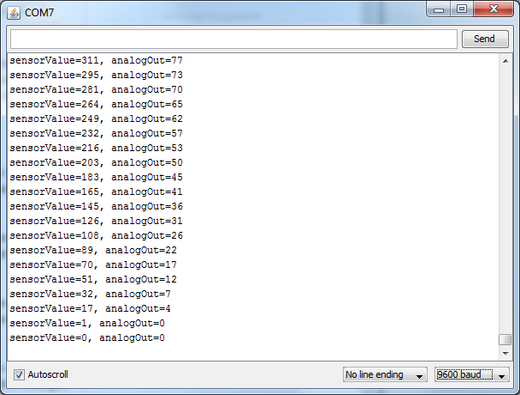
\includegraphics[width=0.5\textwidth]{figures/SM.png}}
\caption{Serial Monitor}
\label{SM}
\end{figure}

Berikan informasi tentang komputer dan informasi komputer Anda tanpa akses ke informasi apa pun terkait penggunaan sistem operasi sistem operasi komputer Arduino. Arduino adalah pengontrol mikro single-board open-source, yang merupakan salah satu platform dengan koneksi kabel, yang akan memungkinkan Anda untuk memasang listrik. AVR Atmel dan perangkat perekaman data yang paling efektif untuk ekspor.
Monitor serial adalah jendela yang menunjukkan data yang dipertukarkan antara arduino dan komputer selama operasi, sehingga Anda dapat menggunakan monitor seri ini untuk menampilkan nilai hasil operasi atau pesan debug. Selain melihat data, Anda juga dapat mengirim data ke Arduino melalui seri monitor ini, dengan memasukkan data dalam kotak teks dan menekan tombol kirim untuk mengirim data. Yang penting untuk diperhatikan adalah menyamakan baudrate antara seri monitor dan papan Arduino.\cite{monk201330}
Untuk menggunakan kemampuan komunikasi serial ini, di Arduino, di bagian kosong dari pengaturan (), ini dimulai dengan instruksi Serial. Diikuti oleh nilai baudrate.
Menulis artikel dan fungsi di perpustakaan arduino adalah: namaobjek.namafungsi
Sebagai contoh, Serial.read (), yang berarti kita memanggil fungsi read () dari objek yang bernama Serial.
Data yang dikirim ke Cisco akan dikirim ke buffer Tx dan informasi yang diterima adalah informasi yang diterima dari penerima buffer (buffer RX).
Jika Anda ingin membuat sebuah template, Anda dapat menggunakan utilitas dari bahas C ++ untuk membuat pustaka untuk semua kelas C ++. Untuk alasan ini, pedoman etika pelanggan yang digunakan untuk mengenali tujuan pemrograman objek. oleh karena itu disarankan sebaiknya anda mempelajari terlebih dahulu hal-hal yang dibutuhkan dalam memahami pemrogaman beroientasi objek.
Arduino kode (sketsa) untuk komunikasi serial akan menjadi mudah karena bekerja di ruang kelas untuk komunikasi serial. Contoh kelas yang digunkan untuk Komunikasi Berkelanjutan (Tujuan) yaitu dengan telah dibuat nama Serial. Untuk arduino dengan lebih dari 1 port serial seperti arduino mega256, nama objek untuk komunikasi serial tersebut adalah Serial1, Serial2, Serial3.z
Buffer adalah area penyimpanan memori ketika dipindahkan antara dua perangkat atau antara perangkat dan aplikasi. Buffering adalah untuk tiga alasan
Alasan pertama adalah untuk memecahkan masalah yang disebabkan oleh perbedaan antara produsen dan konsumen. Misalnya, file diterima oleh modem dan dikirim ke media penyimpanan hard disk. Kecepatan modem sekitar 1/1000 hard drive. Jadi, buffer dibangun ke dalam memori utama untuk menyimpan jumlah byte dari modem. Ketika semua data di clipboard sepenuhnya output, kompresor dapat direkam pada satu disk start-up. Karena teks teks tidak segera tersedia, Anda memerlukan penyimpanan modem, dan kemudian menggunakan 2 buffer. Setelah menjawab interval pertama, disk akan memiliki permintaan tertulis. Modem kemudian mulai merespon buffer kedua, dan buffer pertama digunakan untuk merekam disk. Ketika modem merespon buffer kedua, ia menulis teks perantara pertama, sehingga modem beralih ke interval pertama, yang lain digunakan untuk merekam. Pendekatan dua arah ini meningkatkan jumlah produsen dan konsumen dan mengurangi waktu di antara mereka. Alasan kedua untuk kompresi adalah untuk meningkatkan jangkauan perangkat transmisi data. Interstisial ini sangat banyak digunakan dalam jaringan komputer yang digunakan secara luas untuk berbagi dan mengambil pesan. Di bagian Pengirim, pesan besar dibagi lagi menjadi bagian yang lebih kecil. Koleksi dikirim melalui jaringan, dan penerima menyimpannya di buffer untuk memulihkannya. 
Alasan ketiga untuk kompresi adalah dukungan untuk salinan salinan untuk aplikasi I / O

\subsection {Menulis objek dan fungsi di perpustakaan Arduino dan nama-nama nama dan fungsi}

\begin{figure}[ht]
\centerline{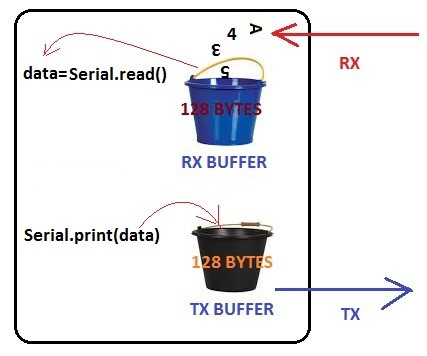
\includegraphics[width=0.5\textwidth]{figures/ember.jpg}}
\caption{Ember}
\label{ember}
\end{figure}

misalnya: Serial.read (), yaitu, objek yang disebut Serial disebut fungsi baca ().
Data yg dikirim  ke serial port  akan dikirim ke buffer pengirim (Tx buffer)  begitupun data yg diterima  adalah data yg diambil  dari  buffer penerima (RX buffer). Data yang dikirimkan berasal dari arduino dalam formulir ASCII. Sebagai contoh, program Arduino untuk mengirim surat yang dikirim ke kode ASCII 1-byte tertentu, atau 65. Jika jumlah 1,2,3, Dikirim mengirim data ASCII 3 byte, yaitu, 49, 48 dan 50. Di sini Anda dapat melihat tabel ASCII berikut:

\begin{table}[H]
\begin{tabular}{|c|c|c|c|c|}
\hline
Dec & Char & Dec Chr & Dec Chr & Dec Chr\\
\hline
16   & DLE (data link escape) & 48 0 & 80 P & 112 p\\
17   & DC1 (device control 1) & 49 1 & 81 Q & 113 q\\
18   & DC2 (device control 2) & 50 2 & 82 R & 114 r\\
19   & DC3 (device control 3) & 51 3 & 83 S & 115 s\\
20	 & DC4 (device control 4) & 52 4 & 84 T & 116 t\\
21	 & NAK (negative acknowledge) & 53 5 & 85 U & 117 u\\
22	 & SYN (synchronous idle) & 54 6 & 86 V & 118 v\\
23	 & ETB (end of trans, block) & 55 7 & 87 W & 119 w\\
24	 & CAN (cancel) & 56 8 & 88 X & 120 x\\
25   & EM (end of medium) & 57 9 & 89 Y & 121 y\\
\hline
\end{tabular}
\end{table}

\begin{figure}[ht]
\centerline{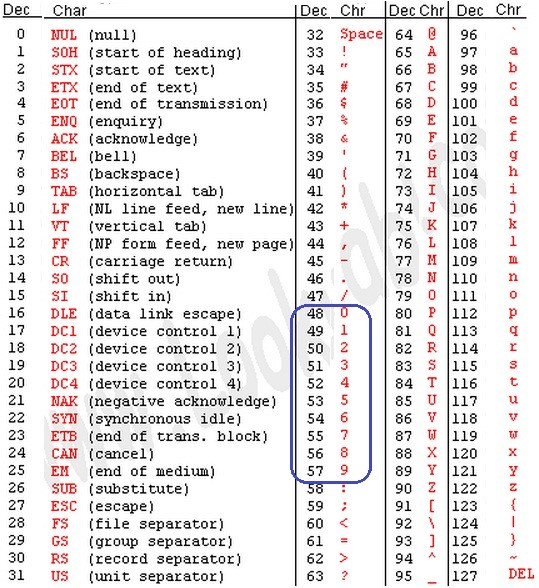
\includegraphics[width=0.5\textwidth]{figures/tabel.jpg}}
\caption{Tabel ASCII}
\label{tabel}
\end{figure}

Karena data yang diperoleh di ASCII (char), kami tidak melakukan matematika data ASCII langsung dalam program sketsa. Data ASCII harus diubah dalam rentang seri terlebih dahulu dengan jumlah form / int. '4' dan '3', '3' + '4' = 103, '3' = 51 dan jika kode ascii '4' = 52 (lihat tabel ASCII).
Konversi data Ascii yang sangat sederhana menjadi data digital, yaitu:
\begin{itemize}

\item untuk mendapatkan angka 0 dari ascii '0' oleh '0'- 48 = 0 (atau bisa juga ditulis' 0 '-' 0 '= 0)
\item untuk mendapatkan nomor 1 dari ascii '1' oleh '1'- 48 = 1 (atau bisa juga ditulis' 1 '-' 0 '= 1)
\item Dll.

\end{itemize}

Jadi kesimpulannya jika Anda ingin menambahkan data ascii '3' dan '4' yang kami terima dari RX Bufer maka kode pemrograman harus:
Int of number = ('3' - '0') + ('4' - '0') atau
int dari angka = ('3'- 48) + (' 4'-48) maka hasil yang diperoleh adalah bilangan bulat 7.
Hal itu dapat mempermudah kamu ketika kamu ingin mengkonversi suatu bilangan yang berbentuk kode ASCII, untuk dapat mengubah suatu bilangan maka diatas telah dijelaskan beberapa cara mudah mengkonversi bilangan ASCII. Sebelum data ASCII dikonversi kepada bilangan tertentu, bilangan harus dirubah terlebih dahulu bentuknya ke dalam bentuk nomor(number) atau integer(int) agar nilai dapat dikonversi secara maksimal.

\subsubsection {Fungsi-fungsi yg tersedia pada serial Arduino}
Semua papan arduino memiliki setidaknya 1 port serial, juga dikenal sebagai UART atau USART. Komunikasi data serial menggunakan 2 pin yaitu pin RX untuk menerima data dan TX ppin untuk mengirimkan data. Di papan arduino pin RX terletak di pin0 dan pin TX terletak di pin1. Ketika papan Arduino dikonfigurasi untuk berkomunikasi secara serial, maka pin0 dan pin1 tidak dapat digunakan sebagai pin input / output digital.Di dalam sistem operasi Windows XP ada program HyperTerminal yang dapat digunakan sebagai alat komunikasi serial dengan perangkat keras. Di Windows yang lebih baru, seperti Win7, Win8 dan Vista, program hyperterminal tidak tersedia. Tapi  program Arduino telah menghadirkan sebuah monitor serial yang dapat dibuka dengan memilih perangkat monitor serial pada menu program arduino.Arduino Nano sudah dilengkapi sebuah port serial yang dapat digunakan melalui port mini usb dengan membuat virtual comport .
Program Arduino telah diselesaikan dengan sebuah pustaka serialport yang memungkinkan pengguna untuk membuat sebuah program baru. Berikut ini adalah beberapa petunjuk yang terdapat dalam pustaka serialport yang dapat digunakan pada papan Arduino Nano.\cite{margolis2011arduino}
\begin{itemize}
\item if (Serial): Untuk memeriksa apakah Port sudah siap
\item Serial.available (): Digunakan untuk memverifikasi apakah ada data yang ada di buffer penerima
\item Serial.begin (): untuk mengatur kecepatan transmisi data
\item serial.end (): Untuk menonaktifkan pin rx dan tx sebagai fungsi serial dan kembali sebagai pin I / O
\item Serial.find (): cari data string dalam buffer
\item Serial.findUntil (): berfungsi untuk mencari buffer data sampai panjang data / terminator yang ditentukan ditemukan
\item Serial.flush (): berfungsi untuk menunggu semua data terkirim
\item Serial.parseFloat (): berfungsi untuk mengambil data float pertama dari data dalam buffer serial.
\item serial.parseInt (): Serial.parseInt (): Serial.parseInt (): Serial.parseInt (): Serial.parseInt (): Serial.parseInt ()
\item Serial.peek (): menampilkan data berikut di buffer penerima
\item Serial.print (): mengirim data ASCII
\item Serial.println (): senddata ASCII + CR, LF (masukkan kode)
\item Serial.read (): membaca data yang diterima
\item Serial.readBytes (): membaca data byte yang diterima
\item Serial.setTimeout (): menetapkan batas waktu maksimum untuk transmisi data.
\item Serial.write (): mengirim data byte (numerik)
\item Serial.serialEvent (): fungsi ini akan dipanggil ketika data tiba / diterima. Kerjanya seperti interupsi serial.
\end{itemize}

\subsection {Langkah untuk membuat program}
Langkah-langkah untuk membuat program sketsa komunikasi serial :

\begin{enumerate}
\item tetapkan baud rate misal 9600 dengan fungsi serial.begin (9600) dalam fungsi void setup (). Kecepatan yang tersedia termasuk 300, 1200, 2400, 4800, 9600, 14400, 19200, 28800,38400, 57600, 115200 (lihat dokumentasi masing-masing jenis arduino).
\item untuk menerima data cek apakah ada data di Rx Buffer dengan fungsi serial.avalable ()
jika data tersedia nilai kembalian = true jika data adalah nilai kembalian kosong = salah.
if (serial.available ()> 0)
\item mengambil data dari penerima buffer: serial.read (), return value adalah 1 byte data pertama di RX Buffer.
misalnya buffer RX byte pertama berisi char 2
kemudian char data = serial.read (); // data = '2' -> karakter
byte data = serial.read (); // data = 50 -> numerik
\end{enumerate}

\begin{itemize}
Untuk mengirim data dapat digunakan
\item serial.print (dataygdikirim): mengirim data ascii
\item serial.println (dataygdikirim), plus masukkan kode (CR dan LF)
\item serial.write (dataygdikirim): mengirim data byte
\item Contoh serial.print ('A') akan mengirim huruf A
\item serial.print (65) akan mengirimkan 2 byte yang berisi kode ascii '6' dan '5' (aktual dikirim 54 dan 53)
\item serial.write (65) akan mengirim 1 byte 65 (aktual yang dikirim numerik 65)
\item serial.write (data) adalah pengganti sintaks Serial.print sebelumnya (data, BYTE). Parameter data dalam serial.write adalah angka 1 byte (0-255)
\end{itemize}

contoh program sketsa sederhana menerima data kemudian data dikirim kembali.


Beberapa contoh yang akan kami buat meliputi:

\begin{itemize}
\item Mengirimkan string data / teks "apa kabar"
\item Mengirim nomor / angka data: 123
\item Menerima data nomor ASCII mis data yang datang misalnya "435"
\end{itemize}

* Langkah yang dilakukan :
karakter diakomodasi dalam array dan dikonversi ke string dengan menambahkan nol 0 ke ujung array (karena string adalah array tipe char yang berakhir dengan null). maka data array / string dikonversi menjadi int dengan fungsi atoi.
Menambahkan port serial pada pin I/O
Jika arduino yg kita miliki hanya punya 1 port serial kita bisa merubah pin I/O yg manapun menjadi Port serial tambahan .dengan bantuan class SoftwareSerial  .  Tambahkan file di header SoftwareSerial.h ke skema dan buat 1 objek SoftwareSerial untuk menambahkan 1 port, dalam contoh di bawah ini, kita akan membuat objek perangkat lunak pihak kedua serial
Pin I / O dapat dimodifikasi oleh portal Port Serial dengan kelas SoftwareSerial. Tambahkan file dalam judul header SoftwareCerial.h dan buat 1 objek SoftwareSerial untuk mengakses 1 port, dalam hal ini kita akan membuat objek perangkat serial 1-serial.
Dapatkan data serial dengan jeda.
pada penerimaan serial interrupt, jika ada data yang datang maka fungsi otomatis serialEvent () akan dieksekusi.\cite{rajamohan2013deaf}